In this chapter, we analyze the third experiment group, that is, the impact of using different scoring techniques in a Blockchain-based Federated Learning system. In this set of experiments, all properties of the system are static, except for the scoring technique, which varies between BlockFlow, Marginal Gain, Multi-KRUM, or none.

\section{Execution Time, Transaction Cost and Latency}

With respect to execution times, we can see on \autoref{tab:metrics_scoring} that every scoring technique gives different results. Since using no scoring technique means that there are less transactions and less computations, it is expected it will be the fastest. That is observable on \autoref{tab:metrics_scoring}, where it is shown that using no scoring technique is twice as fast as most scoring techniques. The fastest scoring technique is Multi-KRUM, taking around $31$ seconds per round; while both BlockFlow and Marginal Gain are the slowest, taking both around $49$ seconds per round.

\begin{table}[!ht]
\centering
\begin{tabular}{c|c|c|c|c} \hline \hline
                               & None   & BlockFlow & Marginal Gain & Multi-KRUM \\ \hline \hline
E2E Time (m)                   & 18.93  & 40.95     & 41.38         & 26.25      \\ \hline
Mean Round Time (s)            & 22.70  & 49.11     & 49.64         & 31.48      \\ \hline
% Median Round Time (s)          & 21.90  & 49.49     & 43.97         & 31.26      \\ \hline
Mean Transaction Latency (s)   & 1.549  & 1.564     & 1.577         & 1.573      \\ \hline
% Median Transaction Latency (s) & 1.549  & 1.558     & 1.564         & 1.551      \\ \hline
Mean Transaction Cost (Gas)    & 183124 & 339645    & 257686        & 280733     \\ \hline
% Median Transaction Cost (Gas)  & 185198 & 189092    & 188994        & 187152     \\ \hline
\end{tabular}
\caption{Time and Transaction Metrics Per Scoring Technique}
\label{tab:metrics_scoring}
\end{table}

We can notice that BlockFlow and Marginal Gain, not only take the longest, but also take a very similar amount of time. As explained in \autoref{background:scoring}, BlockFlow and Marginal Gain scores are computed by other clients, where the Multi-KRUM is computed by the servers. Since the amount of clients is larger than the amount of servers, there are more devices performing scoring computations. For each scoring submission, there is a transaction. The more transactions there are, the more the system has to wait for the blockchain. In addition, clients are usually devices with less computational power. Therefore, it is expected that techniques that run on the clients, such as BlockFlow and Marginal Gain, take longer than techniques that run on the servers, such as Multi-KRUM.

On one hand, we can observe that transaction latency is not influenced by the scoring techniques. The transaction latency, as seen before, is mostly influenced by the consensus algorithm, which, in this case, is static across the experiments. On the other hand, transaction costs are much higher when using a scoring technique. Scoring techniques add at least one more transactions per round per device. Since transaction costs work on a "supply and demand" basis, it is expected that the more transactions are required, the higher the cost will be.

\section{Accuracy and Convergence}

\begin{figure}[!ht]
    \centering
    \centering
    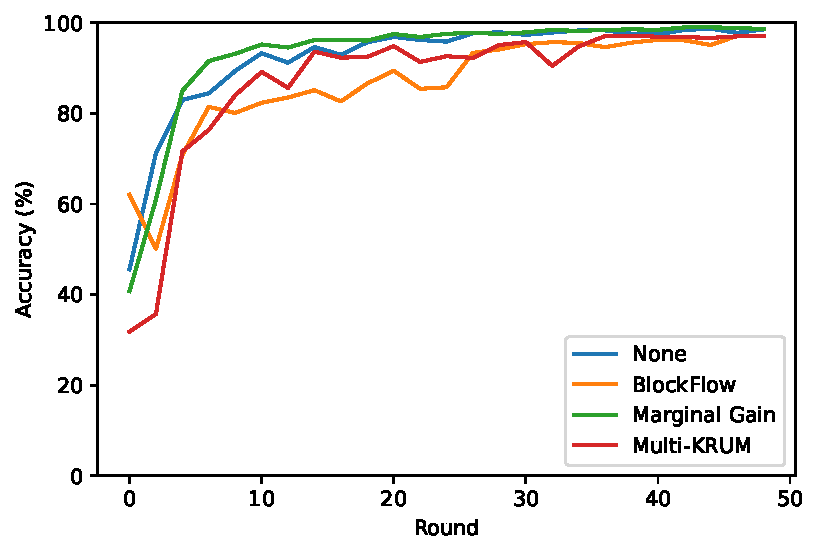
\includegraphics[width=0.7\textwidth]{graphics/scoring/accuracy.pdf}
    \caption{Accuracy Per Scoring Technique}
    \label{fig:accuracy_scoring}
\end{figure}

When comparing the accuracy across the different scoring techniques, we can see on \autoref{fig:accuracy_scoring} that all techniques reached a high accuracy of above $97\%$. However, some techniques reach higher values faster than others, that is, some converge faster than others. As we can see, Marginal Gain converges the fastest, followed by no scoring, then Multi-KRUM and lastly BlockFlow.

On one hand, BlockFlow, is not only the slowest converging scoring technique, but also the only technique that does not drop submissions when aggregating. By not dropping submissions, but still giving them a score that is used during the weighted aggregations, worse submissions are always considered for the global model, which can lead to lower convergence rates. 

On the other hand, Marginal Gain and Multi-KRUM both drop the worst submissions in each round, only considering the best. While Marginal Gain uses its own score for the aggregation, Multi-KRUM uses the amount of samples of each submission, similarly to not using a scoring mechanism. For that reason, Multi-KRUM convergence resembles the one of no scoring mechanism, while Marginal Gain has a smoothest convergence curve.

\section{Communication Costs}

Communication costs also vary massively depending on the scoring technique in use. Some place more strain on the training clients, where others place more strain on the computing servers. On \autoref{fig:net_scoring}, we can visualize the network traffic per round per scoring technique on the clients, servers and blockchain nodes.

\begin{figure}[!ht]
    \centering
    \centering
    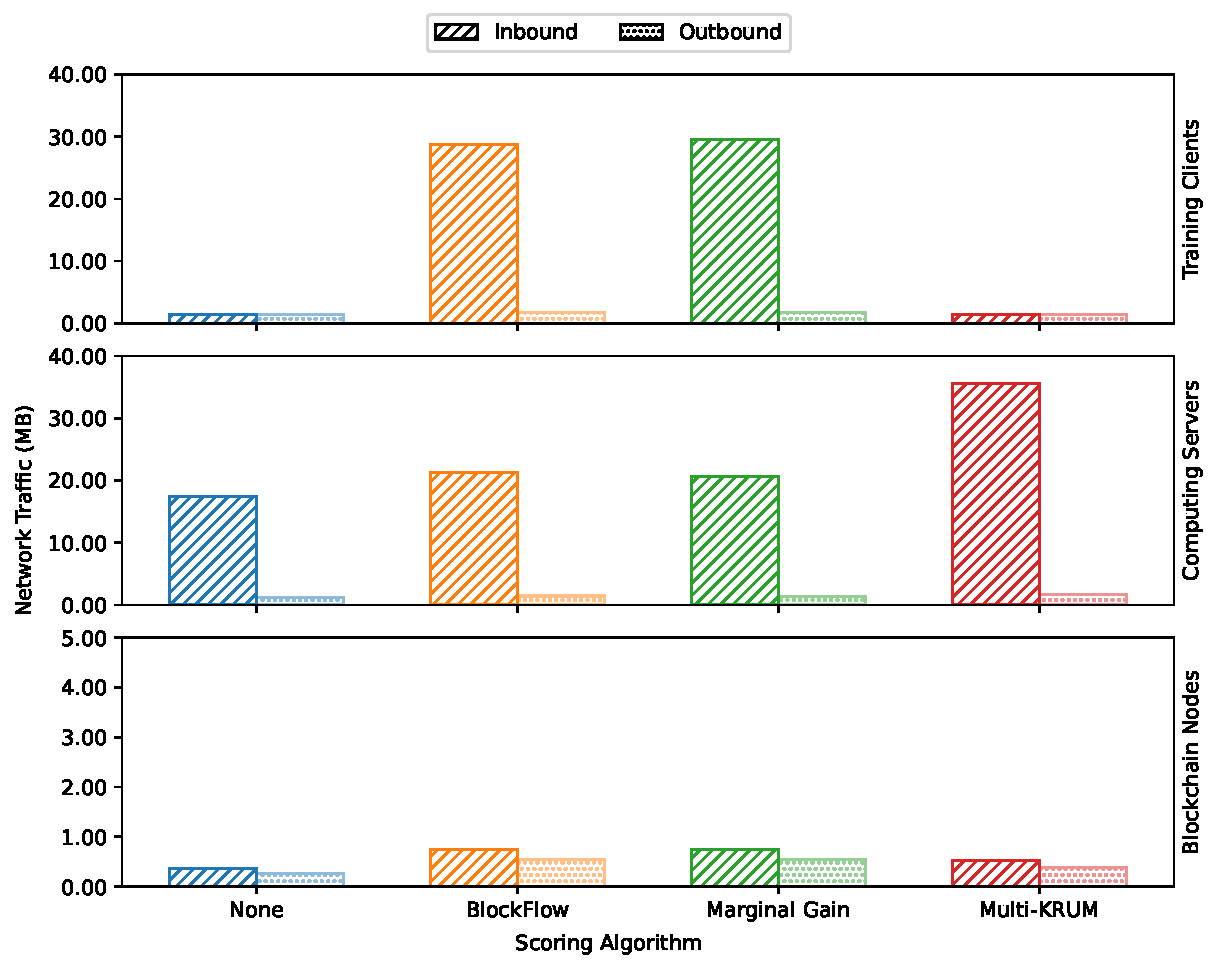
\includegraphics[width=0.8\textwidth]{graphics/scoring/net.pdf}
    \caption{Network Traffic Per Round Per Scoring Technique}
    \label{fig:net_scoring}
\end{figure}

Regarding the training clients, there is a large difference on the network traffic when comparing no technique and Multi-KRUM with BlockFlow and Marginal Gain. On the one hand, Multi-KRUM has similar traffic requirements to using no technique on the clients because the scoring mechanism is executed on the servers. On the other hand, BlockFlow and Marginal Gain require higher levels of inbound traffic, while the outbound traffic remains similar. This phenomenon can be explained by the fact that BlockFlow and Marginal Gain algorithms are executed on the training clients. Since the scoring mechanism is executed on the clients, each client has to download the weights from all the other clients in each round in order to calculate the score, leading to a much higher level of inbound traffic.

Regarding the computing servers, there is not much difference between techniques, except for the Multi-KRUM technique. Multi-KRUM calculates the scores on the server. Therefore, the server has to download the weights of each client's submission an additional time to calculate the scores, compared to the remaining techniques that only download the weights once for the aggregation.

Finally, regarding the blockchain nodes, we can visualize that when using the BlockFlow and Marginal Gain techniques that there is higher network traffic. Multi-KRUM also requires more traffic than no scoring technique, but not as much as BlockFlow or Marginal Gain. This can be explained by the same fact mentioned before: while BlockFlow and Marginal Gain run on clients, Multi-KRUM runs on servers. Since the number of clients is usually higher than the number of servers, there are more transactions when the scoring mechanism runs on the clients. When there are more transactions per round, there is more activity in the blockchain nodes, leading to more network traffic per round.

\section{Computation Costs}

The computation costs across the servers and clients follow a similar trend to what we have seen with the communication costs. On \autoref{fig:ram_scoring} and \autoref{fig:cpu_scoring}, you can visualize the RAM usage, and CPU usage, respectively, on the training clients, computing servers and blockchain nodes during the execution of the experiment.

Regarding the training clients, all techniques require similar amounts of RAM. The techniques that run on the client, Marginal Gain and BlockFlow, consume slightly more RAM, due to having more weights stored in memory, but the difference is negligible when compared to the total amount of RAM it consumes. This can be explained by the fact that the weights are relatively small ($\approx 2$ MB) compared to the total RAM necessary to train a model.

With respect to the CPU consumption, even though it looks similar, it is quite different. On previous analysis, such as in \Cref{chapter:analysis:consensus_algorithms}, we have seen certain techniques end earlier and therefore no data after a certain point. While on those analysis the slower techniques would have high amounts of idle CPU time on the clients, it is not the case here. The techniques that take the longest, that is BlockFlow and Marginal Gain, also have lowest amounts of CPU idle time. This confirms that calculating the scores on the client implies consistently higher CPU usage on the clients.

Regarding the computing servers, it is clear that Multi-KRUM, being the only scoring technique that runs on the server, requires higher amounts of RAM. However, the difference ($\approx 15$ MB) is not significant when considering that the computing servers have large amounts of resources at their disposal. In addition, Multi-KRUM also shows higher levels of CPU consumption, with frequent spikes to $100\%$.

Finally, regarding the blockchain nodes, the difference of CPU and RAM consumption is negligible as expected. Even though the blockchain receives more transactions in total, that does not reflect on the RAM and CPU consumption. The blockchain, by itself, already produces blocks at a constant rhythm. Therefore, the amount of transactions required for the BFL system does not change significantly the consumption.

\begin{figure}[!hpt]
    \centering
    \centering
    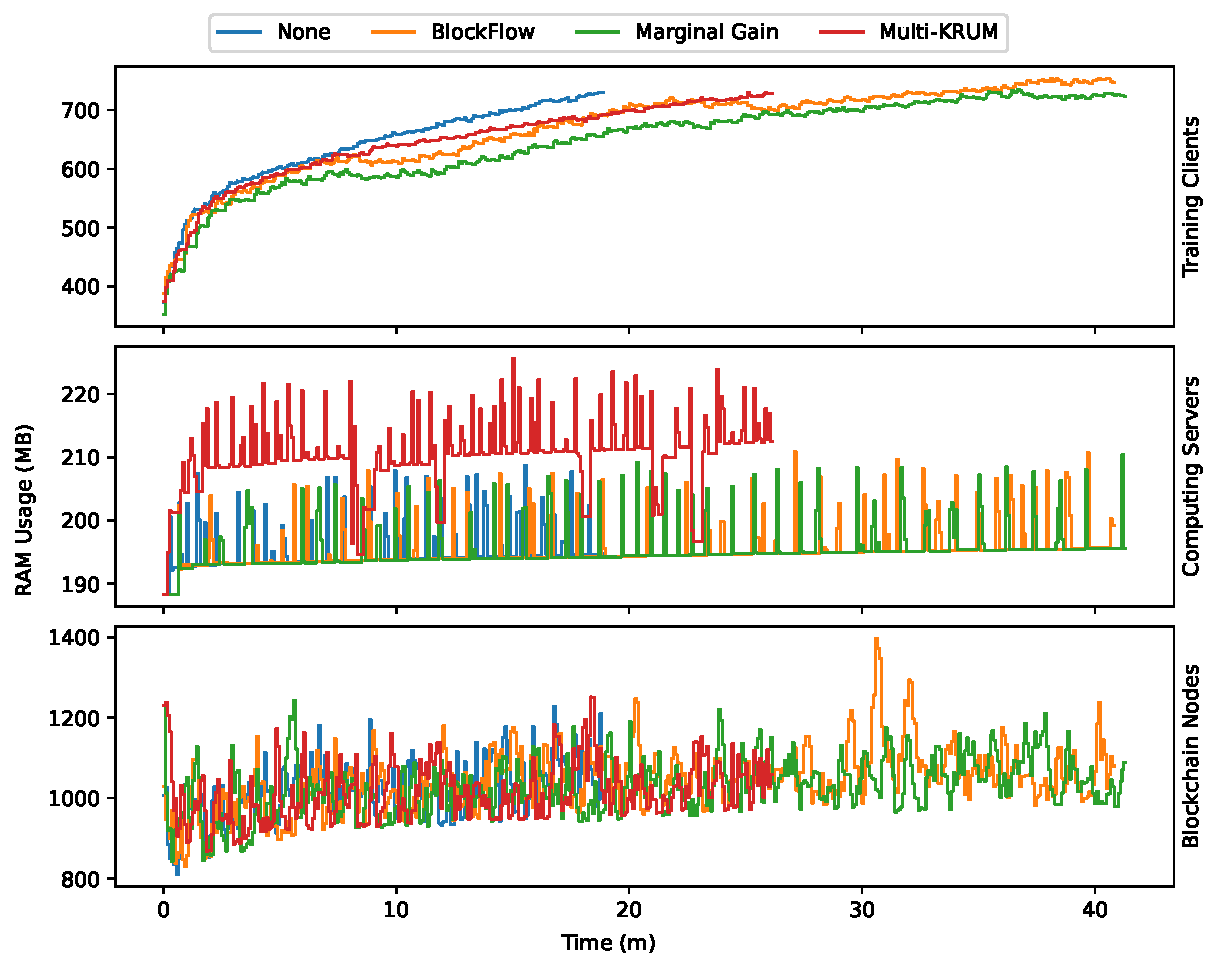
\includegraphics[width=0.8\textwidth]{graphics/scoring/ram.pdf}
    \caption{RAM Usage Per Scoring Technique}
    \label{fig:ram_scoring}
\end{figure}

\begin{figure}[!hpb]
    \centering
    \centering
    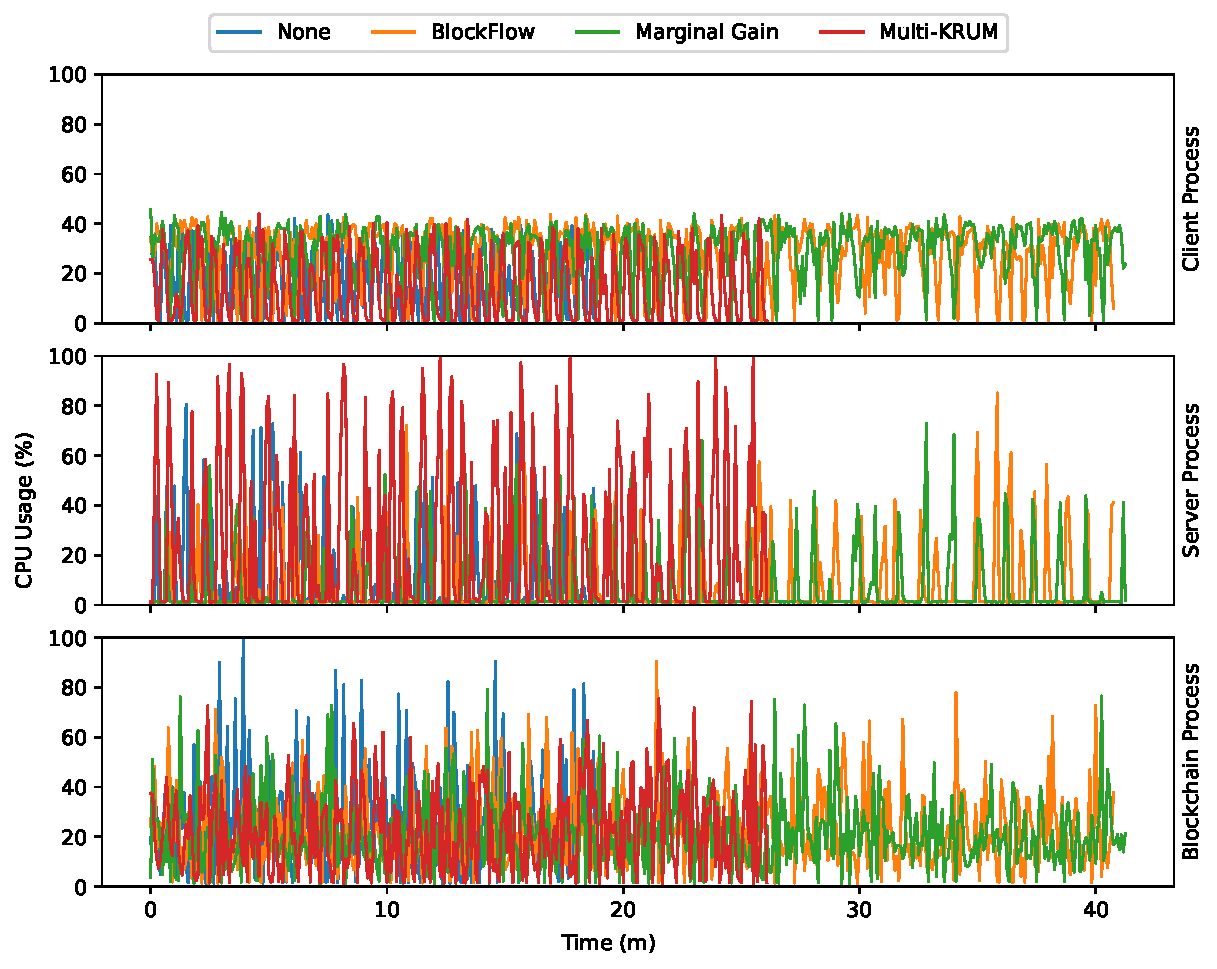
\includegraphics[width=0.8\textwidth]{graphics/scoring/cpu.pdf}
    \caption{CPU Usage Per Scoring Technique}
    \label{fig:cpu_scoring}
\end{figure}

\vfill

\section{Conclusions and Improvements}

In conclusion, scoring techniques that are executed on the clients have a higher impact on the overall system in general, leading to higher round times and higher resource consumption for the clients. In contrast, techniques that are executed on the servers have a higher impact on the servers. Since there is usually a much higher amount of servers than clients, the latter have less impact on the overall system than the former. Additionally, Marginal Gain was the most well performing technique in terms of accuracy and convergence speed, followed by Multi-KRUM and BlockFlow.

If we had to choose between techniques, the choices come down to the priorities of the system. If we are working with a system with low-powered devices, such as IoT systems, it is important that the impact on the clients is lower. Therefore, scoring techniques that run on the server, such as Multi-KRUM, are more valuable. If the opposite is true, or if the resource consumption at the client is not relevant, Marginal Gain could be chosen as it provides the best accuracy of the three.

It is also important to mention that techniques that require more network traffic per round might be slower when using clients with low bandwidth, which is the case of many IoT networks. With lower bandwidths, less traffic can come through at a point in time. Therefore, if there is a high amount of traffic required to be transmitted during a round, devices with low bandwidth can make the process slower.

As a future improvement, servers could cache the information about the weights of the submissions. Specifically, in the Multi-KRUM technique, the servers download each of the client's submission twice: one time for scoring, one time for aggregating. However, the weights downloaded in both of this times are the exact same since they are part of the same round and tied to the same submission. Therefore, caching can work well in favor of reducing the network traffic at the server for this type of techniques.
